\section{Concepts and Used Technologies}
In this section we'll describe and explain the main technologies used in this work.

\subsection{Web Service}
Web Services are a means to enable the interoperability among application components over the Internet.  They are defined as a set of W3C standards, using HTTP for the transport layer and XML serialization for data interchange.

They are  a fundamental component of a programming model called Service Oriented Architecture (SOA). In this model, services are self-describing and self-contained, leading to the development of distributed systems based on loosely-coupled distributed modules.

\paragraph{Interoperability}
When all major platforms could access the Web using Web browsers, different platforms could interact. For these platforms to work together, Web-applications were developed. Web-applications are simple applications that run on the web. These are built around the Web browser standards and can be used by any browser on any platform.

\paragraph{Reusable application-components}
There are things applications need very often. So why make these over and over again? Web services can offer application-components like: currency conversion, weather reports, or even language translation as services.

\paragraph{Connect existing software}
Web services can help to solve the interoperability problem by giving different applications a way to link their data. With Web services we can exchange data between different applications and different platforms. \citep{WST}

\subsubsection{Technologies}

\paragraph{Extensible Markup Language (XML)}
is a set of rules for encoding documents in machine-readable form. It is defined in the XML 1.0 Specification produced by the W3C, and several other related specifications. It provides a language which can be used between different platforms and programming languages, and still express complex messages and functions.

\paragraph{Hypertext Transfer Protocol (HTTP)} 
is the most used Internet protocol, this way one does not get restrained with firewalls, for instance.

\paragraph{Web Service Description Language (WSDL)}
is an XML format for describing network services as a set of endpoints operating on messages containing either document-oriented or procedure-oriented information. The operations and messages are described abstractly, and then bound to a concrete network protocol and message format to define an endpoint. Related concrete endpoints are combined into abstract endpoints (services). WSDL is extensible to allow description of endpoints and their messages regardless of what message formats or network protocols are used to communicate.

\subsection{Orchestration}
Orchestration describes how web services can interact with each other at the message level, including the business logic and execution order of the interactions. These interactions may span applications and/or organizations, and result in a long-lived, transactional, multi-step process model. In this model of service composition, there is a central node that controls the logic of the entire process. This node has the responsibility to manage the process, choosing which services will be invoked, how messages are exchanged between these services and how to proceed with the possible exceptions and failures. Figure \ref{BPELexample} shows the message exchange between a client, a travel agency (the central node) and two web services.

\begin{figure}[htb]
  \centering
  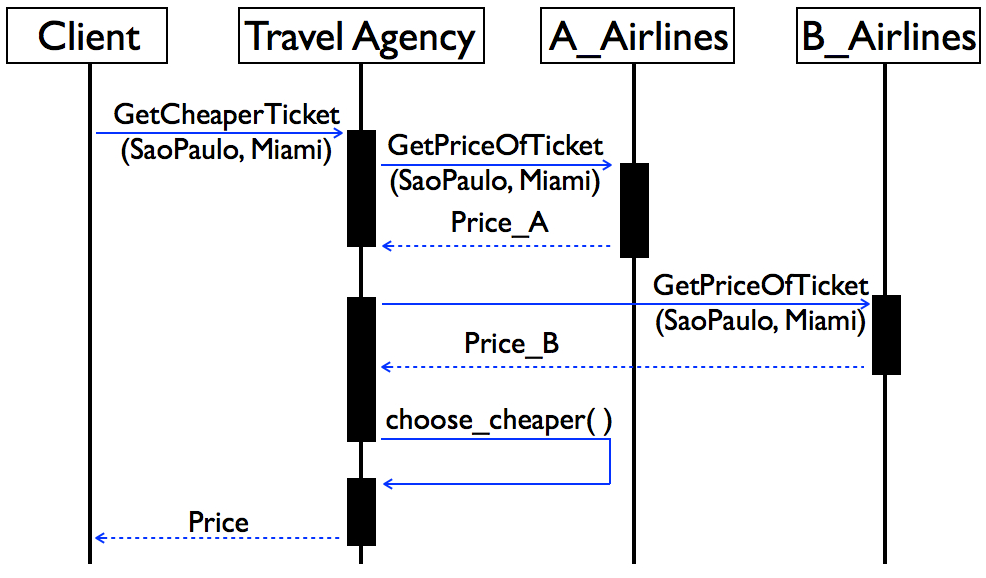
\includegraphics[width=\textwidth]{images/BPELexample}
  \caption{BPEL example flow}
  \label{BPELexample}
\end{figure}

Orchestration is not defined as a W3C standard. It's standardized by OASIS. The co-chair of the Web Service Choreography working group of W3C (in 2005), Steve Ross-Talbot, said that ``OASIS is a very different kind of organization. By contrast, it's much more vendor-led than the W3C. The W3C is responsible for all the core building blocks of the Web, for Web services and for the semantic Web. All the ancillary things you need to make Web services happen, such as management and orchestration, are in OASIS''. \citep{INTERVIEW}

But the fact is that the industry is embracing orchestration as the way to specify, generate and control business process built upon web services. This was an initiative of IBM with Microsoft to develop a unified standard for Orchestration.

Basically, one must first describes the orchestration through a XML document, then generate an executable process from this file, and finally execute the process. A good analogy would be a \emph{C} program, with only the main function (orchestration definition) that uses a lot of functions (operations) of included libraries (partner web services). The hole logic is embedded in this one description, the central node. 

Historically (2002), three standards arose from the cooperation between companies, e.g. IBM, Microsoft, Sun, BEA, and others, interested on the development of the Web:

\paragraph{BPEL4WS} 
stands for ``Business Process Execution Language for Web Services'', the specification — called BPEL, for short — models the behavior of Web services in a business process interaction. It provides an XML-based grammar for describing the control logic required to coordinate Web services participating in a process flow. The WSDL interface defines the specific operations allowed, and BPEL defines how to sequence them. BPEL is a layer on top of WSDL. The WSDL interface defines the specific operations allowed, and BPEL defines how to sequence them. WSDL describes the public entry and exit points for every BPEL process, and WSDL data types describe the information that passes between process requests. Additionally, WSDL can reference external services that the BPEL process requires. A simple BPEL model can be found at \ref{BPELstructure}.

\begin{figure}[htb]
  \centering
  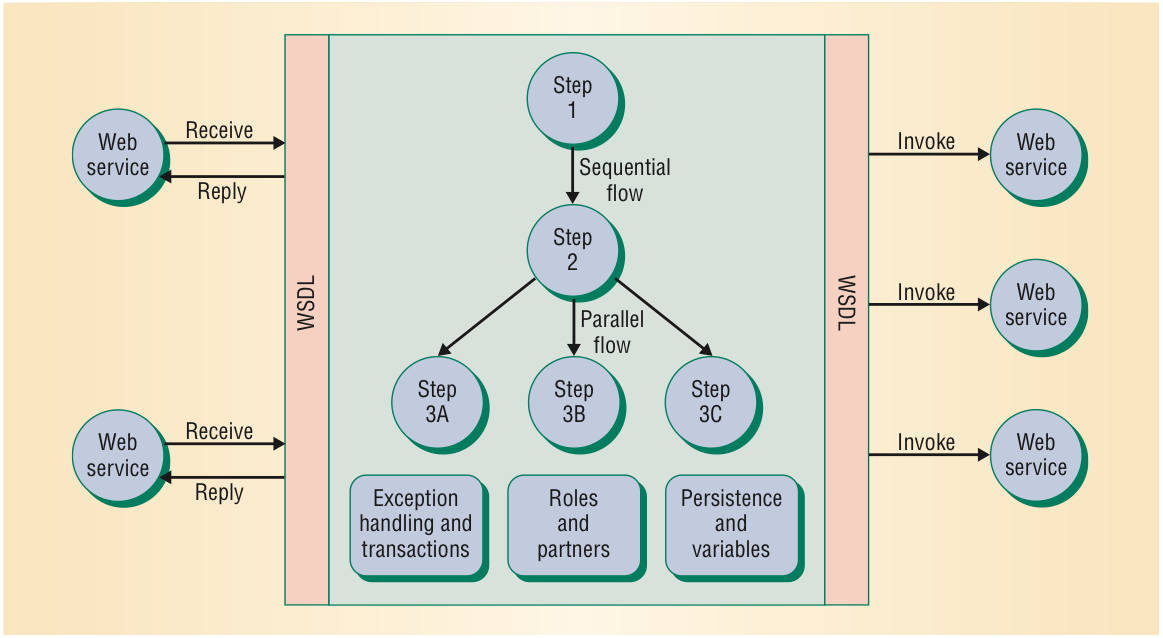
\includegraphics[width=\textwidth]{images/BPELstructure}
  \caption{BPEL structure}
  \label{BPELstructure}
\end{figure}

\paragraph{WSCI}
is the ``Web Service Choreography Interface''. It defines a collaboration extension to WSDL, describing only the observable behavior between Web services. It does not address the definition of executables business process as BPEL does.

\paragraph{BPML} 
the ``Business Process Management Language'' also incorporate WSCI support. BPML and WSCI share the same underlying process execution model, so developers can use WSCI to describe public interactions among business process and reserve BPML for developing private implementations.

In the beginning of 2003, all the companies supporting BPML discontinued it's support, migrating to BPEL4WS. It became a standard by OASIS, whom renamed the standard to ``WS-BPEL'', the change was made to align with others Web Services standards of the organization. \citep{OASIS}

Nowadays the main standard is still BPEL, with a lot of tools to write it's definition. But even though there is a lot of good tools for modeling the process (e.g. NetBeans, Eclipse, Petals studio, Orchestra, and many others), there aren't many good tools for it's deployment. We started using Apache's ODE to execute the process, then migrated to Orchestra, finally succeeded with Netbeans, but this last required a graphical environment to execute. So we finally discovered PEtALS ESB. 

\subsubsection{Tools}

\paragraph{Eclipse}
is one of the most popular Java IDE in the market. It's plugin architecture allows it to become an IDE for anything. With BPEL Designer plugin, Eclipse enhance the ability to display and edit BPEL workflows with a graphical UI.

\paragraph{NetBeans}
as Eclipse, netbeans is originally a Java IDE founded at plugins. The enterprise version 6.5 brought a bundle to use with Web Services and Orchestration. This was another graphical designer for BPEL, but the code it produced was readable and editable to human beens, so we used this to generate the base orchestration to the generator

\paragraph{Apache ODE}
is a WS-BPEL compliant web services orchestration engine. It organizes web services calls following a process description written in BPEL. Another way to describe it would be a web service capable workflow engine. This engine is the most used open source orchestration engine for orchestration available, but apache's license isn't compatible with GPL, so we preferred to search other tool before using it.

\paragraph{Orchestra}
is another open source BPEL engine. It's license is LGPL, compatible with ours, but we couldn't find an easy way to deploy the services there.

\paragraph{PEtALS ESB}
is an Open Source Enterprise Service Bus for large SOA architectures. \citep{PEtALS} An ESB is a tool that integrates existing services or applications, exposed to the Bus as a service, using standard service languages resulting in greater adaptability and automation. PEtALS ESB also has a module for executing BPEL. This way we were able to create synthetical services in each node of the Bus and execute the composition on Amazon Elastic Compute Cloud (Amazon EC2).



\subsection{Choreography}
Web Service Choreography is a form of service composition in which there is no single node that controls the entire process, i.e., control is distributed throughout the system. In a choreography, the interaction protocol among several partner services is defined from a global perspective. At run-time, each participant in a choreography performs a role and interacts with its neighboring participants. As there is no single point of control, and therefore, no single point of failure, there is a better potential for building scalable systems than in the case of centralized orchestrations.

The name of the composition came from the analogy of the process with dancers. While in an orchestra there is the Conductor that sets the timing and rhythm, in a group of dancers there is no coordinator during the enactment, the people only reacts to neighbors to perform it's role.

There have been a few attempts to create standards:

\paragraph{WS-CDL}
stands for ``Web Services Choreography Description Language'', is a W3C candidate recommendation. It is a language for describing how peer-to-peer participants collaborate. The language uses XML, and some aspects are inspired by the pi-calculus

\paragraph{WSCI}
as mentioned earlier, it defines a nut shell around the WSDL description of the Web Service.

\paragraph{BPMN}
``Business Process Modeling Notation'' is a graphical representation for specifying business processes in a business process model. The new version (2.0), still in beta phase, has a set of construct blocks to specify choreography process. this new version will also have execution semantics, which will enable the future development of tools to enact choreographies.

Although there was those attempts by the W3C and OMG to specify standard languages to define choreographies, up to the moment there are no implementations that allow the enactment of choreographies specified in standard languages.

Choreographies and Orchestration can relate to each other as represented in Figure \ref{relation-orchestrationXchoreography}.


\begin{figure}[htb]
	\centering
	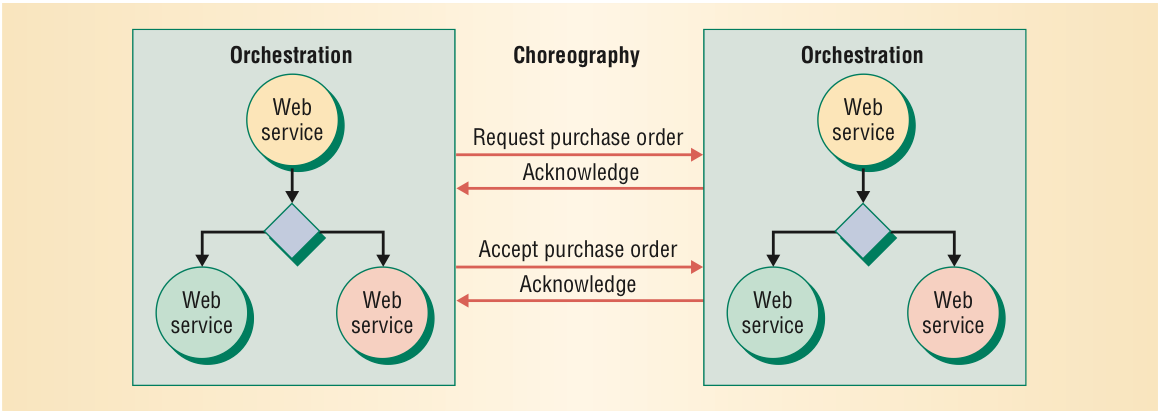
\includegraphics[width=\textwidth]{images/relation-orchestrationXchoreography}
	\caption{Relationship between Orchestrations and Choreographies}
	\label{relation-orchestrationXchoreography}
\end{figure}




\subsection{Cloud Computing}
More recently, a new generation of middleware systems and hardware infrastructures were developed to cope with other kinds of applications requiring large processing power. In this case, the motivation was end-user applications such as email, office suites, calendars, and many other e-commerce, social networks, and Web 2.0-style applications used daily by hundreds of millions of users. Large Internet-based companies such as Amazon and Google used virtualization technologies to develop the basis for what was later called Cloud Computing \citep{ZCB10}. Google App Engine provides an execution environment for Web applications that can then be executed in the hardware infrastructure provided by Google; developers can write applications in Java or Python and use standard APIs for storage and communication.  The Amazon Elastic Compute Cloud or EC2 \citep{EC2} provides a virtual computing environment in which developers can instantiate multiple virtual machines booting, from scratch, standard operating systems such as GNU/Linux or Windows. These sets of machines can then run any application developed for these operating systems. When necessary, the developer can also create an image from a current instance of his virtual machines set and then create new instances with the given image, shortening the configuration time for these new machines.